\section{Time Dilation from Vortex Dynamics}\label{sec:Part-1}

    We consider an inviscid, irrotational superfluid æther with stable topological vortex knots. Absolute time $t_{\text{abs}}$ always ticks constant, while local clocks might experience slowed rates due to pressure gradients and knot energetics. The Vortex Æther Model posits that the rate at which time flows in the local frame (near the knot) depends on the internal angular frequency $\Omega_k$. In this section, we derive time dilation analogues inspired by the predictions of general relativity (GR), based solely on pressure and vorticity gradients in the fluid.

\begin{figure}[h!]
    \centering
    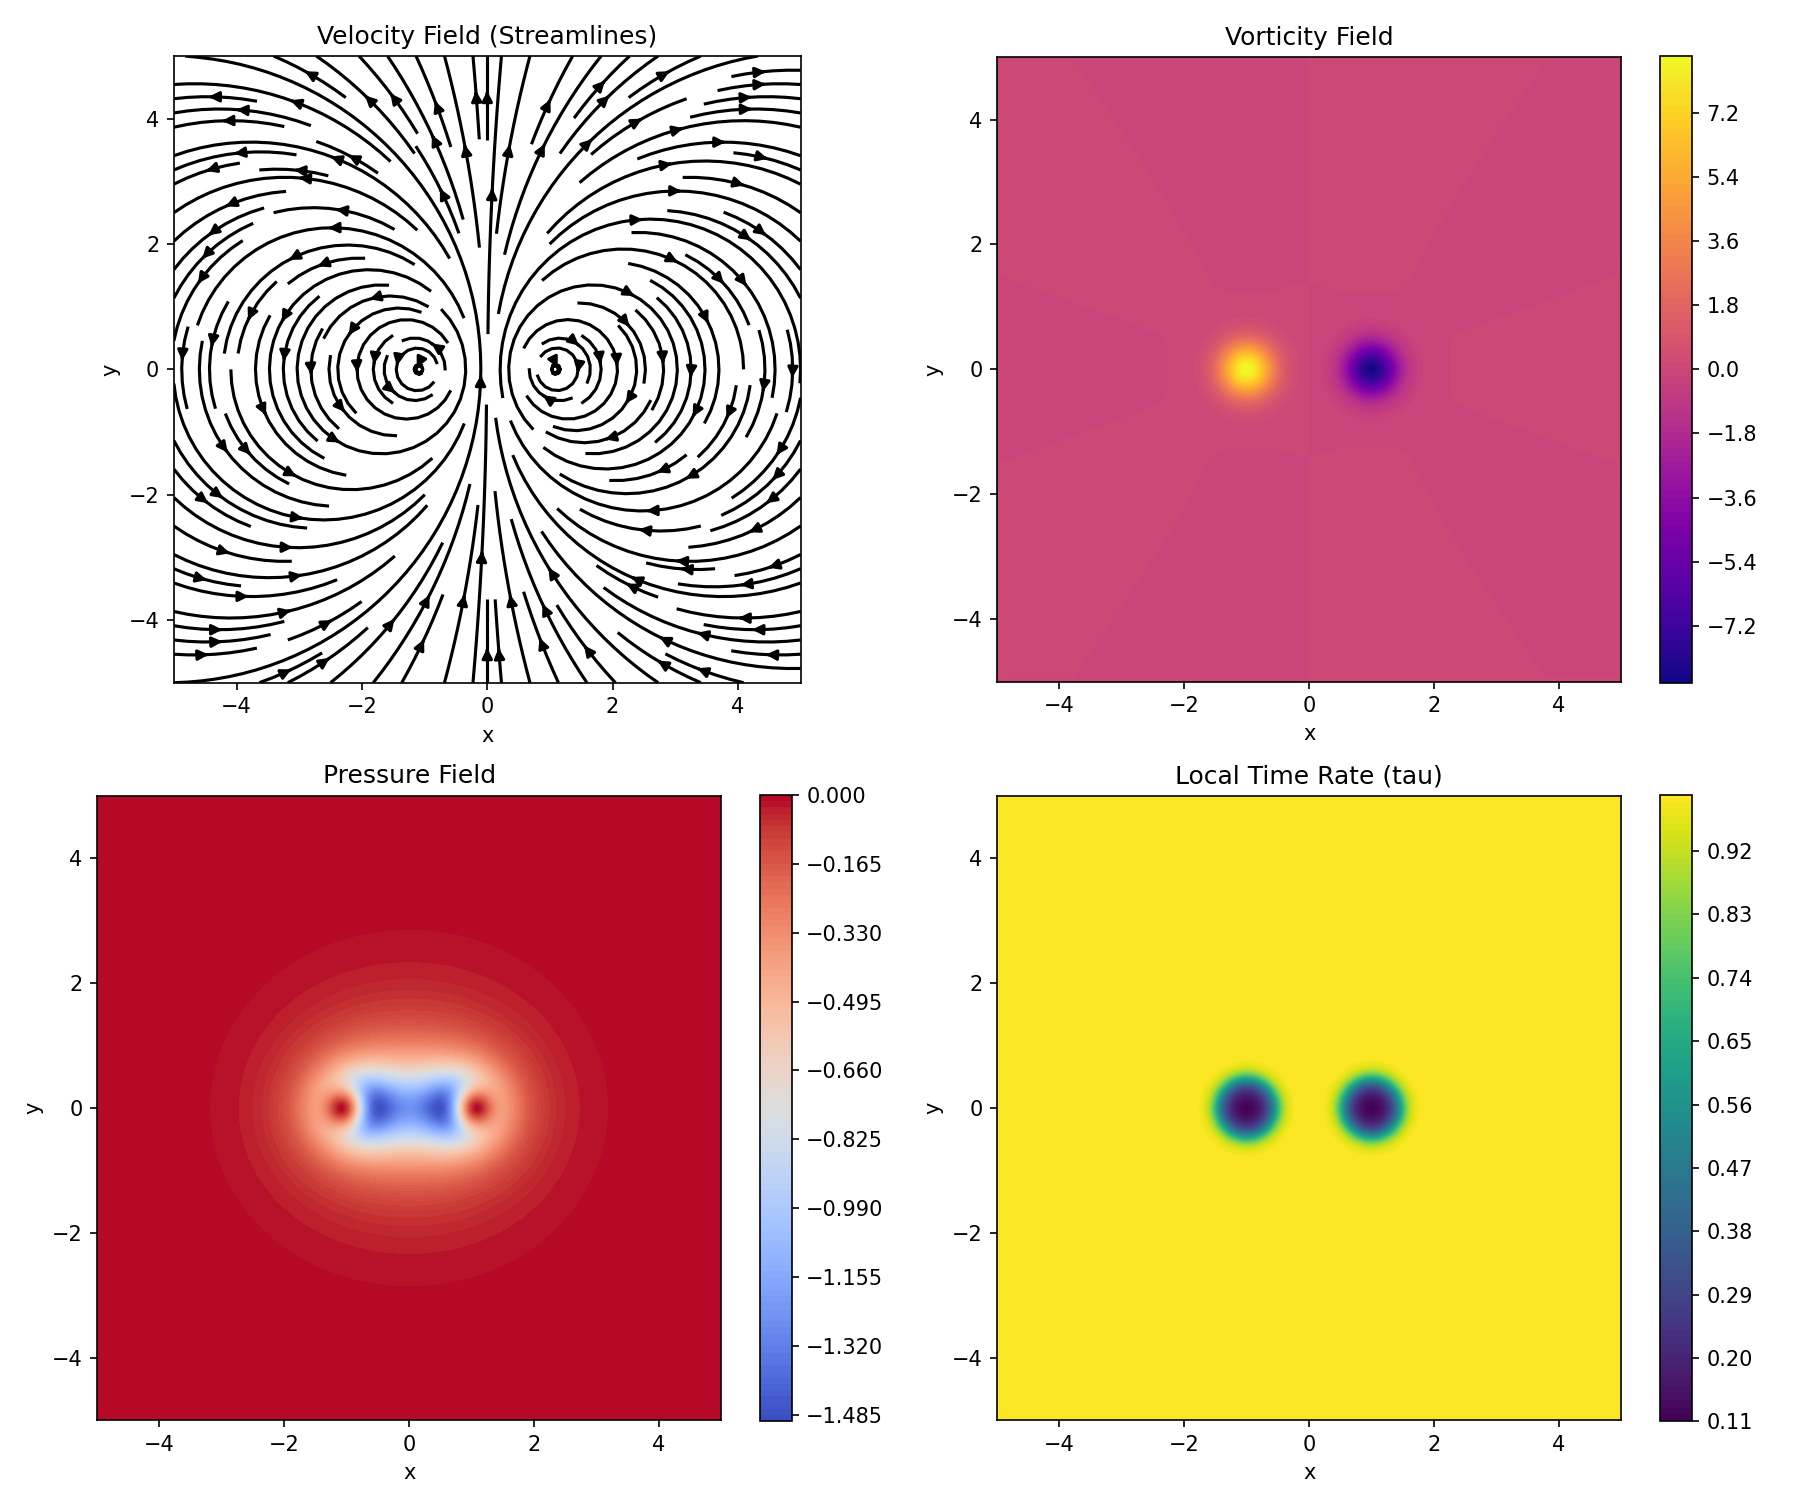
\includegraphics[width=0.85\textwidth]{export/streamlinesDiPole}
    \caption{Velocity streamlines, vorticity, pressure, and local time rate $\tau$ for a simulated vortex pair. The pressure minimum and time slow-down clearly align with the regions of high vorticity. This directly illustrates the æther model's central claim: time dilation follows from vortex energetics and pressure depletion.}
    \label{fig:vortexfields}
\end{figure}

\subsection*{A. Bernoulli Flow and Local Time Depletion}

In a classical, inviscid, incompressible fluid, Bernoulli's equation describes the conservation of energy in a flow:

\begin{equation}
    \frac{1}{2} \rho_{\text{\ae}}  v^2 + p = p_0 \Rightarrow p = p_0 - \frac{1}{2} \rho_{\text{\ae}} v^2
\end{equation}

Here:
\begin{itemize}
    \item $p_0$ is the background reference pressure,
    \item $\rho_{\text{\ae}}$ is the constant æther density,
    \item $v$ is the local velocity of the æther near the vortex.
\end{itemize}

Assuming that clock rate is proportional to pressure (i.e., time slows in low-pressure regions), we relate the local clock frequency to the background as:

\begin{equation}
\frac{f_{\text{local}}}{f_0} = 1 - \frac{\rho_{\text{\ae}} v^2}{2 p_0}
\end{equation}

Hence, time dilation is:

\begin{equation}
    \frac{t_{\text{local}}}{t_0} = \left(1 - \frac{\rho_{\text{\ae}} v^2}{2 p_0}\right)^{-1}
\end{equation}

For rotational flow, with $v = \Omega r$,

\begin{equation}
    \frac{t_{\text{local}}}{t_0} = \left(1 - \frac{\rho_{\text{\ae}} \Omega^2 r^2}{2 p_0} \right)^{-1} \approx 1 + \frac{\rho_{\text{\ae}}\Omega^2 r^2}{2 p_0}
\end{equation}

This expression recovers the first-order time dilation analog if we define the dimensionless coupling:

\begin{equation}
    \frac{\rho_{\text{\ae}}}{p_0} \sim \frac{1}{c^2}
\end{equation}

This motivates the analogy to relativistic time dilation:

\begin{equation}
    \frac{t_{\text{moving}}}{t_\text{rest}} \approx 1 + \frac{v^2}{2 c^2}
\end{equation}

\begin{figure}[h!]
    \centering
    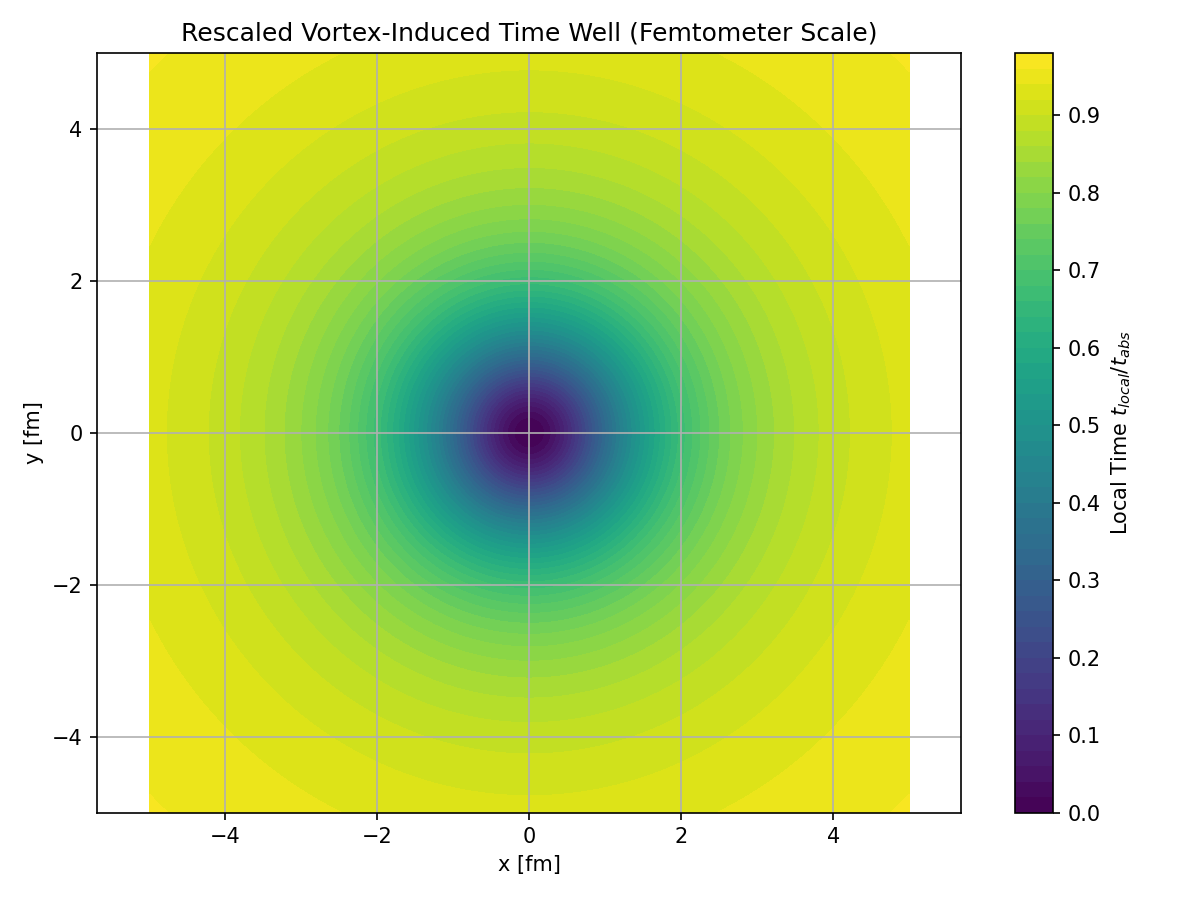
\includegraphics[width=0.8\textwidth]{export/RadialProfileOfLocalTimeDilation_Vortex-Induced_Time_Well}
    \caption{Schematic of a vortex-induced time well in the æther. Local time $t_{\text{local}} / t_{\text{abs}}$ is shown as a color gradient in 2D space. The central vortex region exhibits the most time slowing due to high $\Omega_k$, forming a well-like structure.}
    \label{fig:vortex_time_well}
\end{figure}


\subsection*{B. Heuristic Knot-Based Time Modulation}

Topological vortex knots have intrinsic angular frequency $\Omega_k$, conserved due to vorticity confinement. We introduce a first-principles motivated
time dilation expression:

\begin{equation}
\frac{t_{\text{local}}}{t_{\text{abs}}} = \left(1 + \alpha \Omega_k^2 \right)^{-1}
\end{equation}

where $\alpha$ is a coupling parameter with dimensions $[\alpha] = \text{s}^2$. Expanding for small $\Omega_k$:

\begin{equation}
\frac{t_{\text{local}}}{t_{\text{abs}}} \approx 1 - \alpha \Omega_k^2 + \mathcal{O}(\Omega_k^4)
\end{equation}

This form mirrors the expansion of the Lorentz factor:

\begin{equation}
\frac{t_{\text{moving}}}{t_{\text{rest}}} \approx 1 - \frac{v^2}{2 c^2}
\end{equation}

\begin{figure}[h!]
    \centering
    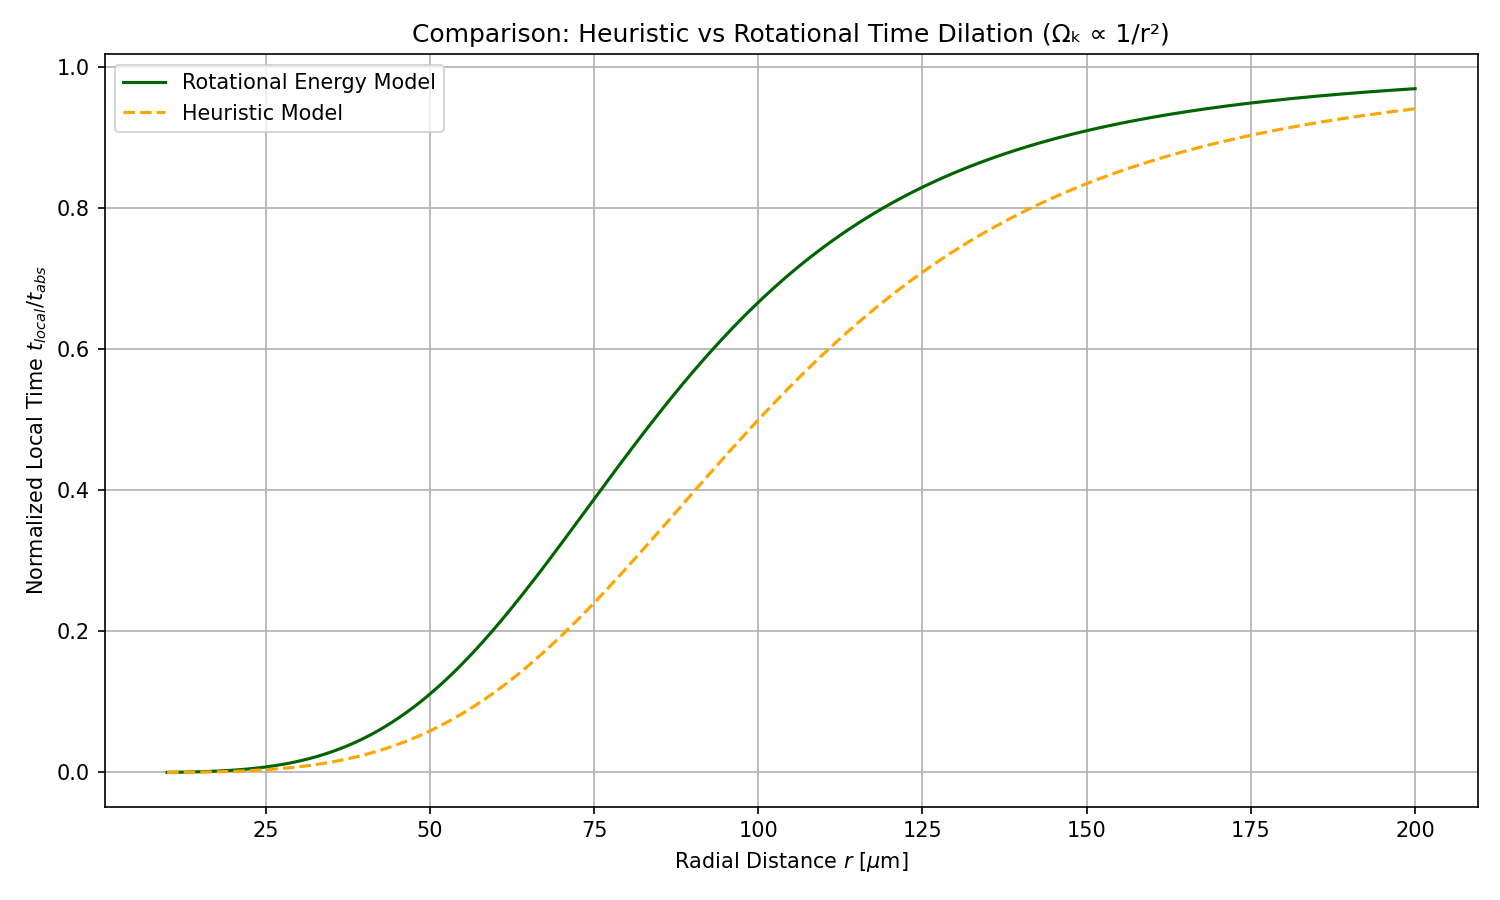
\includegraphics[width=0.8\textwidth]{export/RotationalVsHeuristicTimeDilation}
    \caption{\textbf{Comparison: Heuristic vs Rotational Time Dilation (\(\Omega_k \propto 1/r^2\))}.
    This graph compares two models of time modulation within the Vortex Æther framework.
    The heuristic model (green) assumes time rate reduction proportional to \((1 + \alpha \Omega_k^2)^{-1}\),
        while the rotational model (dark blue) incorporates rotational energy \(E_{\text{rot}} = \frac{1}{2} I \Omega_k^2\) and suppresses local time via
        \((1 + \frac{1}{2} \alpha I \Omega_k^2)^{-1}\). Both curves exhibit strong time dilation near the vortex core (\(r \sim 10^{-15}\) m),
        approaching absolute time flow only at extended distances. The rotational model yields a steeper suppression,
        highlighting the energetic cost of maintaining high angular momentum in fluid-based time curvature.
    }
    \label{fig:radial_time_profile}
\end{figure}

\subsection*{C. Time Dilation from Rotational Inertia}

We now ground the heuristic form in physical energetics. For a knot with moment of inertia $I$, the rotational energy is:

\begin{equation}
E_{\text{rot}} = \frac{1}{2} I \Omega_k^2
\end{equation}

Thus, the time dilation becomes:

\begin{equation}
\frac{t_{\text{local}}}{t_{\text{abs}}} = \left(1 + \alpha E_{\text{rot}} \right)^{-1} = \left(1 + \frac{1}{2} \alpha I \Omega_k^2 \right)^{-1}
\end{equation}

This boxed equation is the core result of this section:

\begin{equation}
\boxed{\frac{t_{\text{local}}}{t_{\text{abs}}} = \left(1 + \frac{1}{2} \alpha I \Omega_k^2 \right)^{-1}}
\end{equation}

\subsection*{D. Summary of Model Hierarchy}

\begin{itemize}
\item Pressure-Based (Bernoulli): Time slows in low-pressure zones due to vortex velocity.
\item Heuristic Angular Model: Time slows as a function of $\Omega_k^2$.
\item Energetic Model: Time flow depends on stored rotational energy in the knot.
\end{itemize}

These form a continuum of physical justification, culminating in a replacement of spacetime curvature with rotational æther mechanics. This establishes the VAM time dilation framework as a fluidic, topologically-conserved analog to GR.

Next, we will explore how these models correspond to GR-like metrics and rotational observers in Section II.